% This text is proprietary.
% It's a part of presentation made by myself.
% It may not used commercial.
% The noncommercial use such as private and study is free
% Sep. 2010
% Author: Sascha Frank 
% University Freiburg 
% www.informatik.uni-freiburg.de/~frank/
%
% 

\documentclass[handout]{beamer}
\setbeamertemplate{navigation symbols}{}


\usetheme{Warsaw}
\usepackage{ngerman}
\usepackage{media9}
\usepackage[utf8]{inputenc}
\beamersetuncovermixins{\opaqueness<1>{25}}{\opaqueness<2->{15}}
\begin{document}
\title{LES RESEAUX DOMESTIQUES}  
\author{LAVIER Antoine et NTUMBA wa NTUMBA Patient}
\date{\today} 

\begin{frame}
\titlepage
\end{frame} 

\begin{frame}
\frametitle{Contenu}
\tableofcontents
\end{frame} 


\section{Exemple de réseau domestique}
\begin{frame}\frametitle{Exemple de réseau domestique} 
\begin{figure}
		\centering
		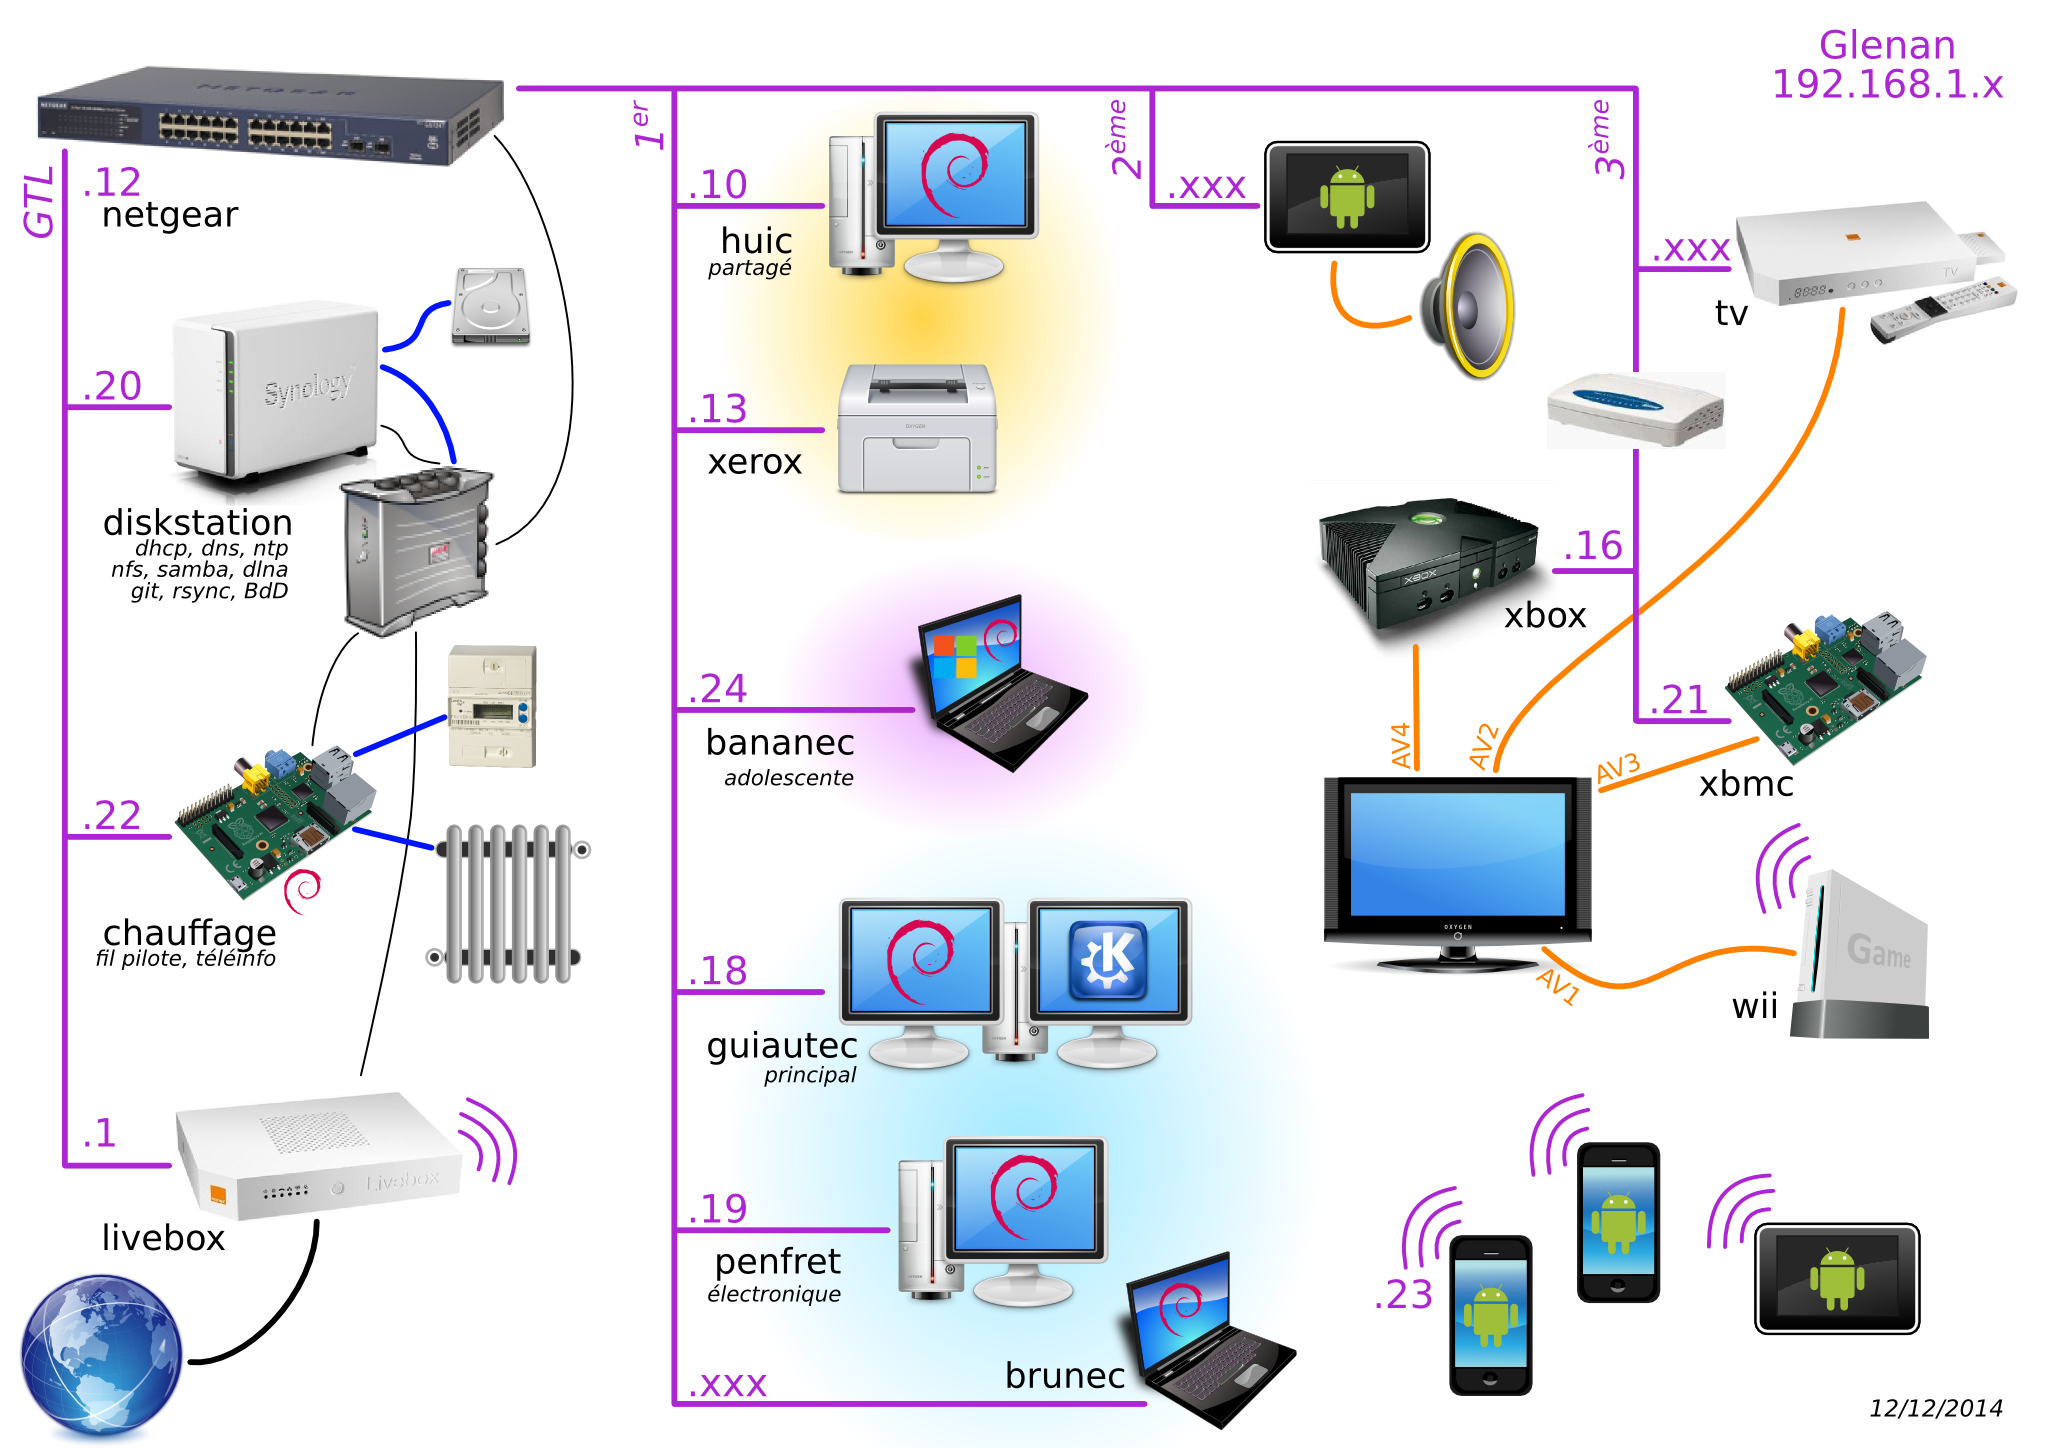
\includegraphics[width=\textwidth,height=0.8\textheight,keepaspectratio]{image/LAN6.png}
\end{figure}
\end{frame}

\section{Appareils d'un réseau domestique}
\begin{frame}\frametitle{Appareils du réseau domestique} 
\end{frame}

\subsection{Insfrastructure}
\begin{frame}\frametitle{Insfrastructure} 
\end{frame}

\section{Les services dans un réseau domestique}
\begin{frame}\frametitle{Les services dans un réseau domestique} 
\end{frame}

\section{La domotique dans un réseau domestique}
\begin{frame}\frametitle{La domotique dans un réseau domestique} 
\end{frame}

\section{Et la maison du futur}
\begin{frame}\frametitle{La domotique dans un réseau domestique} 
\begin{figure}
    \centering
    \includemedia[
    width=0.6\linewidth,height=0.3375\linewidth,
    activate=pageopen,
    flashvars={
        modestbranding=1 % no YT logo in control bar
        &autohide=1 % controlbar autohide
        &showinfo=0 % no title and other info before start
        &rel=0 % no related videos after end
    }
        ]{}{https://www.youtube.com/watch?v=TptZ8m8prd4}
\end{figure}
\end{frame}
\end{document}
